%\VignetteIndexEntry{Oligo Vignette}
%\VignetteDepends{oligo}
%\VignetteKeywords{Expression, SNP, Affymetrix, NimbleGen, Oligonucleotide Arrays}
%\VignettePackage{oligo}
\documentclass{article}

\newcommand{\Rfunction}[1]{{\texttt{#1}}}
\newcommand{\Rmethod}[1]{{\texttt{#1}}}
\newcommand{\Rcode}[1]{{\texttt{#1}}}
\newcommand{\Robject}[1]{{\texttt{#1}}}
\newcommand{\Rpackage}[1]{{\textsf{#1}}}
\newcommand{\Rclass}[1]{{\textit{#1}}}
\newcommand{\oligo}{\Rpackage{oligo }}

\usepackage{graphicx}

\usepackage{/home/bst/student/bcarvalh/bin/R-2.5.0/share/texmf/Sweave}
\begin{document}
\title{An Introduction to the Oligo Package}
\date{March, 2007}
\author{Benilton Carvalho}
\maketitle


\section{Introduction}

The \oligo package is designed to support all microarray designs
provided by Affymetrix and NimbleGen: expression, tiling, SNP and exon
arrays. With the increase in the density of the current technologies,
\oligo uses the resources offered by the \Rpackage{BufferedMatrix}
packages to handle the feature-level information. As of now,
chip-specific packages are built via \Rpackage{makePlatformDesign} and
transitioning to the \Rpackage{pdInfoBuilder} package, which creates
the data packages for the Affymetrix SNP arrays.

\section{Analyzing Affymetrix SNP Arrays}

Genotyping can be performed using \oligo and you will need:

\begin{itemize}
\item \oligo and its dependencies;
\item Chip specific data package, eg. \Rpackage{pd.mapping50k.xba240}:
  package that contains the array specifications and SNP annotation.
\item CEL files.
\end{itemize}

Figure \ref{workflow} shows the general workflow for genotyping using
the \oligo package. 

\begin{figure}[h]
  \centering
  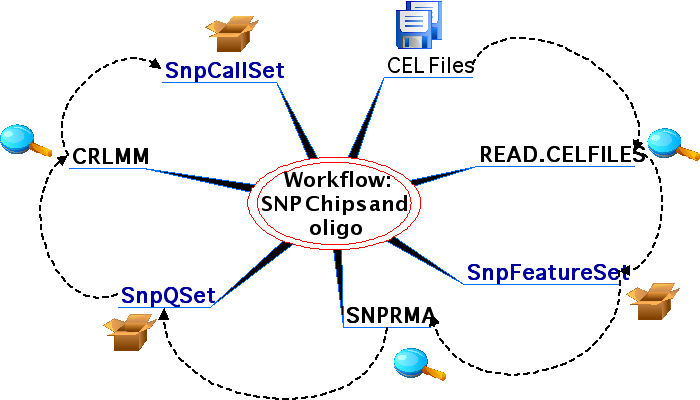
\includegraphics[scale=.5]{workflow.png}
  \caption{Genotyping workflow using the \oligo package.}
  \label{workflow}
\end{figure}

We will start by loading the \oligo package and importing the CEL
files available on the \Rpackage{sampleDataAffy100K}. The intensity
matrix will be a \Rclass{BufferedMatrix} object and this will require
the use of temporary files in order to reduce the RAM usage. Although
the temporary files can be stored anywhere, a better approach will be
to use a local directory rather than using a directory on the
network. The \Robject{tmpdir} in the \Rfunction{read.celfiles()} sets
the directory where the temporary files are going to be stored.

\begin{Schunk}
\begin{Sinput}
R> library(oligo)
R> library(hapmap100kxba)
R> pathCelFiles <- system.file("celFiles", package = "hapmap100kxba")
R> fullFilenames <- list.celfiles(path = pathCelFiles, 
     full.names = TRUE)
R> temporaryDir <- tempdir()
R> rawData <- read.celfiles(fullFilenames, tmpdir = temporaryDir)
\end{Sinput}
\begin{Soutput}
Incompatible phenoData object. Created a new one.


Welcome to the pd.Mapping50K_Xba240 prototype pdInfo package
WARNING: DO NOT USE THIS PACKAGE FOR ANY ANALYSIS.
THIS PACKAGE IS FOR INTERFACE PROTOTYPE USE ONLY!
THE DATA HAS NOT BEEN VALIDATED AND LIKELY HAS ERRORS.
Have fun!
\end{Soutput}
\end{Schunk}

The \Robject{rawData} object is of class \Rclass{SnpFeatureSet}, which
extends \Rclass{eSet}. Methods like \Rmethod{exprs()} and
\Rmethod{pm()} are defined and, again, return \Rclass{BufferedMatrix}
objects.

The \Rclass{phenoData} slot includes covariates about the
samples. Genotyping and copy number analyses often make use of gender
information in order to provide more precise inferences. The code
below exemplifies the creation of the \Rclass{phenoData} object.

\begin{Schunk}
\begin{Sinput}
R> aboutSamples <- data.frame(gender = c("female", 
     "female", "male"))
R> rownames(aboutSamples) <- sampleNames(rawData)
R> aboutVars <- data.frame(labelDescription = "male/female")
R> rownames(aboutVars) <- "gender"
R> phenoData(rawData) <- new("AnnotatedDataFrame", 
     data = aboutSamples, varMetadata = aboutVars)
\end{Sinput}
\end{Schunk}

Preprocessing SNP arrays can be done by using the \Rfunction{snprma()}
method, described in \cite{Carvalho2006}. Once it is completed, an
\Rclass{SnpQSet} object is returned, which is the summarized data of the
\Robject{rawData} object above. An overview of the method is presented
at Figure \ref{snprma}.

\begin{figure}[h]
  \centering
  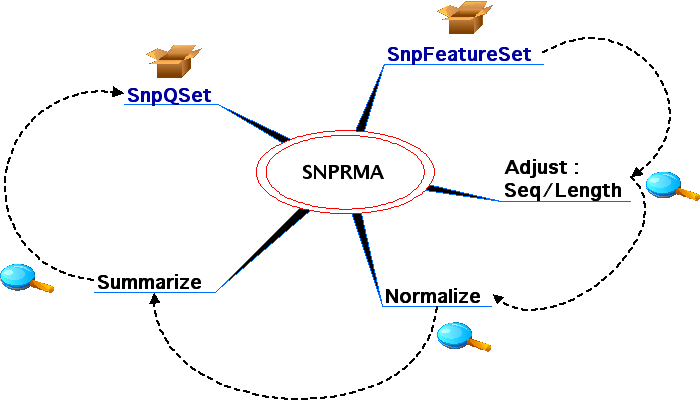
\includegraphics[scale=.5]{snprma.png}
  \caption{SNPRMA overview}
  \label{snprma}
\end{figure}

For each SNP there are four numbers $(\theta_{A-}, \theta_{B-},
\theta_{A+}, \theta_{B+})$, which are proportional to the
log-intensities in each of these combinations of allele and strand
($-$: antisense; $+$: sense). They are represented by four matrices:
\Robject{antisenseThetaA}, \Robject{antisenseThetaB},
\Robject{senseThetaA} and \Robject{senseThetaB}, which are the
components of the \Rclass{SnpQSet} object. One can extract these
objects using accessors of the same name.

Average intensities and log-ratios are defined as across allele and
within strand, ie:
\begin{eqnarray}
  A_{s} & = & \frac{\theta_{A, s}+\theta_{B, s}}{2} \\
  M_{s} & = & \theta_{A, s} - \theta_{B, s},
\end{eqnarray}
where $s$ defines the strand (antisense or sense). These quantities
can be obtained via \Rmethod{getA()} and \Rmethod{getM} methods, which
return high-dimensional arrays with dimensions corresponding to SNP's,
samples and strands, respectively.
\begin{Schunk}
\begin{Sinput}
R> preProcessedData <- snprma(rawData)